\documentclass{article}
\usepackage[utf8]{inputenc}
\usepackage{graphicx}
\usepackage{float}
\usepackage{verbatim}
\usepackage{subfiles} 
\usepackage{fancyhdr}
\usepackage{hyperref}
\usepackage{natbib}
\usepackage{xparse}
\usepackage{xcolor, soul} 

\NewDocumentCommand{\codeword}{v}{%
"\textbf{\texttt{#1}}"
%\fcolorbox{black}{lightgray}{\texttt{\textcolor{darkgreen}{#1}}}%
}


\title{DevOps, Software Evolution \& Software Maintenance Rapport}
\author{Course code: KSDSESM1KU\\\\
Group O - Oh sorry\\\\
Repository: \url{https://github.com/Group-O-Minitwit/minitwit-group-o}
\\\\
Christoffer Tofteng (chtof@itu.dk)\\German Alexander Garcia Angus (gega@itu.dk)\\Hristiyana Hristova Toteva (hrto@itu.dk)\\Lasse Emil Sonn (lson@itu.dk)\\Mikkel Munkholm Blak Nilsson (muni@itu.dk)\\Nohely Gedeon (noho@itu.dk)}

\date{May 2023}

%REMEMBER MAX 3500 WORDS
\pagestyle{fancy}
\fancyhf{}
\rhead{Group O - chtof, gega, hrto, lson, muni \& noho}
\lhead{DevOps Rapport}
\rfoot{Page \thepage}

\begin{document}
\maketitle
\newpage
\tableofcontents
\newpage

\section{Introduction}
This paper aims to describe the our experience on working with development of the simplified twitter clone - MiniTwit. Our primary focus has been on designing a reliable system, which is transparent and easy to maintain.
\section{System's Perspective}
\subsection{Design of the systems}
We have designed our system in a monolithic structure\footnote{Awati et al.} where all our components are build and deployed together. The system has been separated into smaller components in order to maintain a loosely coupled application. These components consist of a frontend system, a remote server, a database, a monitoring system, and a logging system.
\subsection{Architecture of the systems} 
Our version of the MiniTwit application consists of a web application, an API, and a database. The application is inspired by Twitter. It allows users to create a profile, log in, post short messages to a public timeline, and follow and unfollow other users. The web application is supported by our API, which has endpoints to handle those functionalities. The frontend was developed using the JavaScript React.js library with Node.js as the runtime environment. The API was built with C\# using the .Net framework. A more in-depth discussion as to why we chose these technologies for our system can be found in section \ref{technologies}.

\begin{figure}[H]
    \centering
     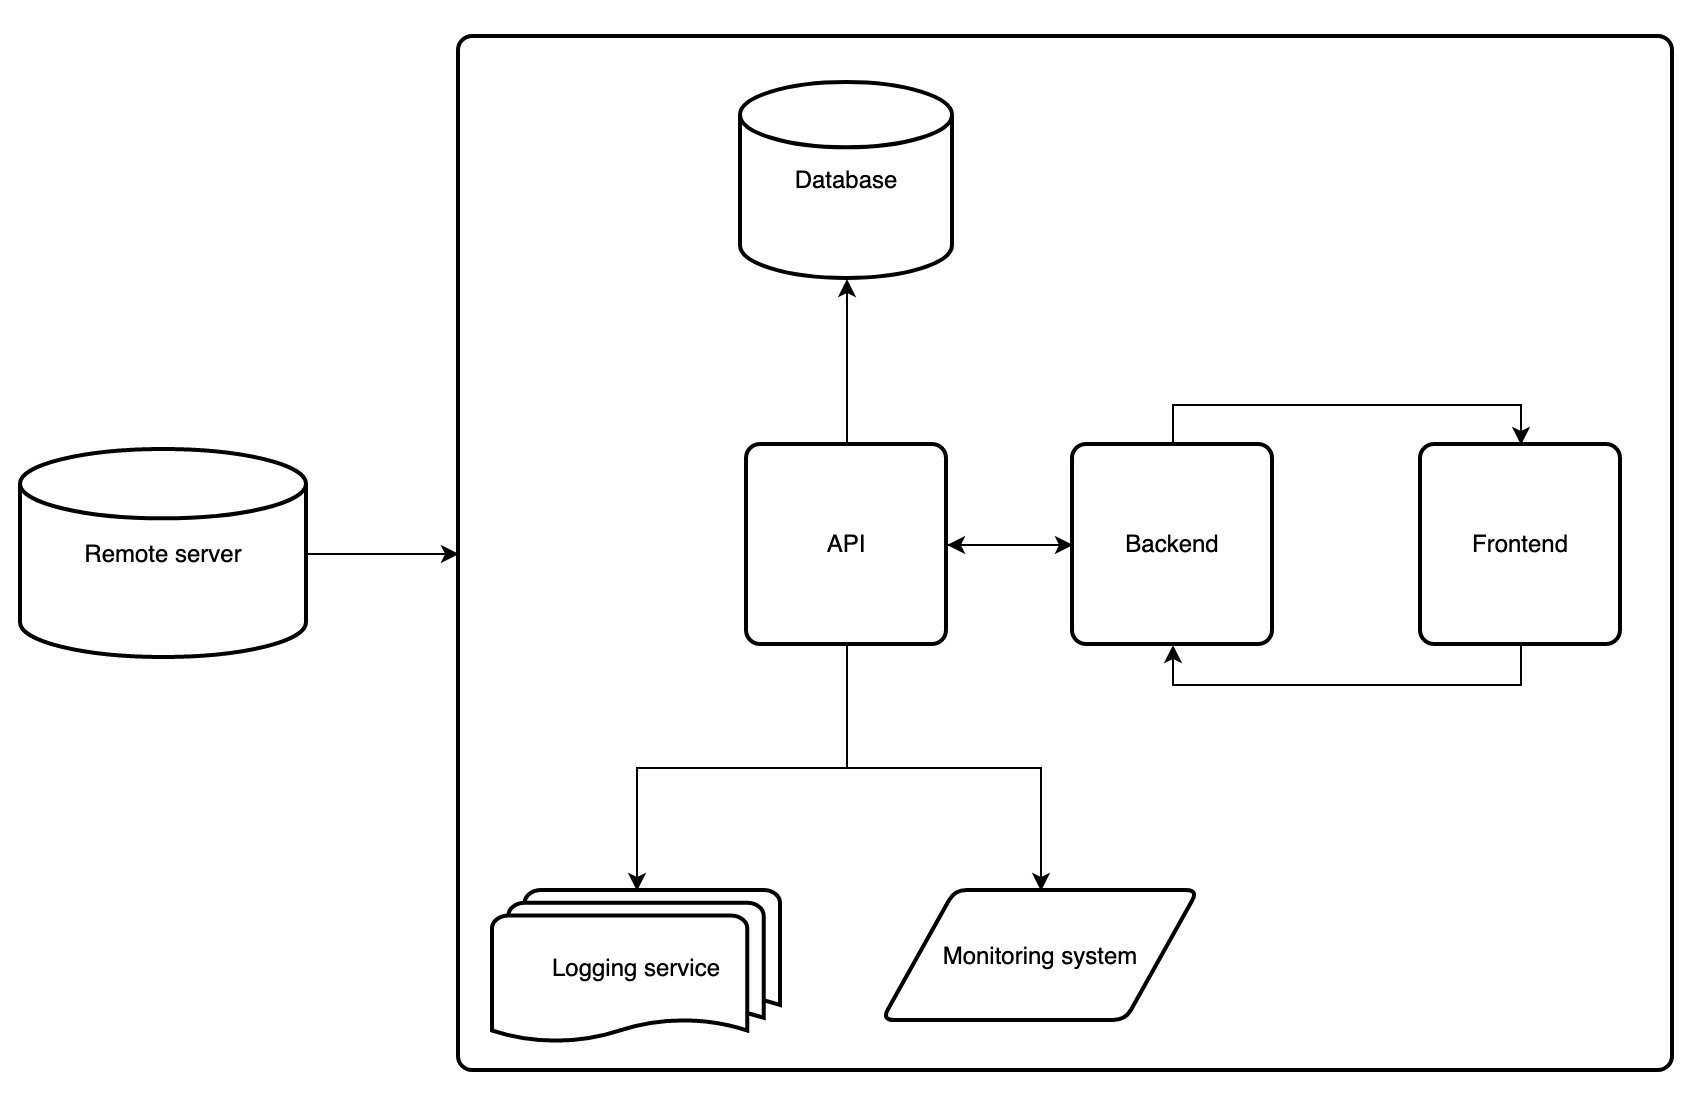
\includegraphics[width=\textwidth]{images/Software_architecture.png}
    \caption{Architecture of our software}
    \label{fig:architecture}
\end{figure}

\subsection{Dependencies}
For a visualization of the dependencies please see figure \ref{fig:dependencies}
\begin{itemize}
    \item \textbf{C\#} \cite{Csharp}\\
    We use C\# and the .NET framework to handle all the API and data manipulation in our application. 
    \item \textbf{React} \cite{react}\\
    The React library is used to visualize our data through the frontend with JavaScript
    \item \textbf{PostgreSQL} \cite{postgresql}\\
    We're using PostgreSQL as our database system.
    \begin{itemize}
        \item \textbf{npgsql} \cite{npgsql}\\
        The database for our project is NPGSQL which is a .NET version of a Postgres database.
    \end{itemize}
    \item \textbf{Prometheus} \cite{prometheus}\\
    Prometheus collects and stores the metrics of our application. The metrics can be access with Prometheus's queries that help to connect with the Grafana monitoring tool. 
    \item \textbf{Grafana} \cite{grafana}\\
    To visualize and analyze our monitoring data we are using Grafana, which shows different metrics that can be access by using the Prometheus's queries.
    \item \textbf{SeriLog} \cite{seriLog}\\
    SeriLog is a C\# logging tool that creates logs and formats them before sending them to ElasticSearch.
    \item \textbf{ElasticSearch} \cite{elasticsearch}\\
    This tool is a data ingestion toool used to index the logs send from SeriLog in order to allow for easier access.
    \item \textbf{Kibana} \cite{kibana}\\
    Kibana is used to query the logs from ElasticSearch and visualize the data from the log.
    \item \textbf{filebeat} \cite{filebeat}\\
    Filebeat is a logshipper used to ship the logs to elasticsearch
    \item \textbf{nginx} \cite{nginx}\\
    We are using the proxy service nginx for port forwarding in relation to our logging.
    \item \textbf{Docker} \cite{docker}\\
    We're using docker to containerize our application. This is done to keep the setup intuitive and makes it easy to do continuous deployment. Together with docker we're specifically using docker-compose which helps centralize the setup to a single yaml file.
    \item \textbf{DigitalOcean} \cite{digitalocean}\\
    DigitalOcean is used to host the server which runs our application. The server is running an image of Ubuntu 22.04 with Docker preinstalled. Together with this we have a static IP with locks our application to a specific IP, so we have the possibility to change the remote server but keep the same IP.
    \item \textbf{GitHub Actions} \cite{ghactions}\\
    Github Actions is used for the CI/CD pipeline.
    \item \textbf{Static analysis tools}
    We have InferSharp, CodeQL and SonarCloud running in our CI/CD chain to ensure software quality in what we are committing to the project.
    \begin{itemize}
        \item \textbf{InferSharp} \cite{infersharp}\\
        InferSharp is the C\# version of the static analytic tool Infer used by Facebook. InferSharp both analysizes for null dereferences, resource leaks, and thread-safety violations and has a security check for the likes of SQL injections.
        \item \textbf{CodeQL} \cite{codeql}\\
        CodeQL is a static analytics tool that run through the code and treats it like data. Therefore it is possible to also make CodeQL custom queries, however, we did not make use of that feature as our codebase is not that big and complex and the standard analysis is enough.
        \item \textbf{SonarCloud} \cite{sonarcloud}\\
        SonarCloud is a quality measuring tool to give your committed code a grade based on some predefined parameters that may or may not be relevant. In our case it checks for duplicated lines, "smelly" code, some security and reliability. In addition to the two "heavier" analyzers, we think SonarCloud seems like a solid one to handle the things that the two first does not.
    \end{itemize}
\end{itemize}

\begin{figure}[H]
    \centering
     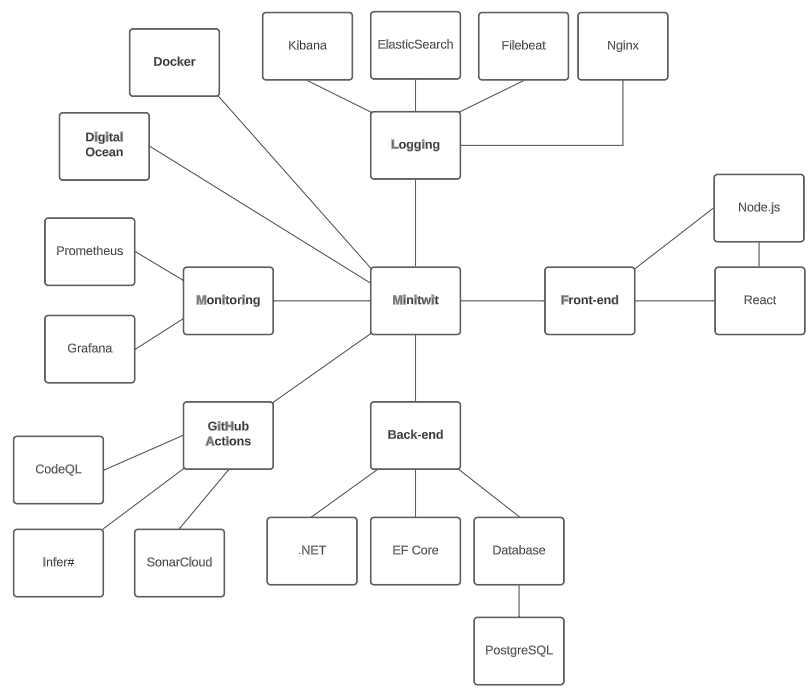
\includegraphics[width=\textwidth]{images/dependencies.png}
    \caption{Structure of our dependencies}
    \label{fig:dependencies}
\end{figure}

\newpage
\subsection{Important interactions of subsystems}
Given that the frontend is built independently from our API with the frontend being React and the API being C\# the frontend accesses endpoints of the API in order to visualize the data and send new data if a new tweet or  user is created. 
\subsection{Current state of the system}
The only tool we use that can really give us a current picture of our system is SonarCloud. As you can see on figure \ref{fig:sonarcloud} below we get the grade A based on the parameters we have chosen. 
\begin{figure}[H]
    \centering
     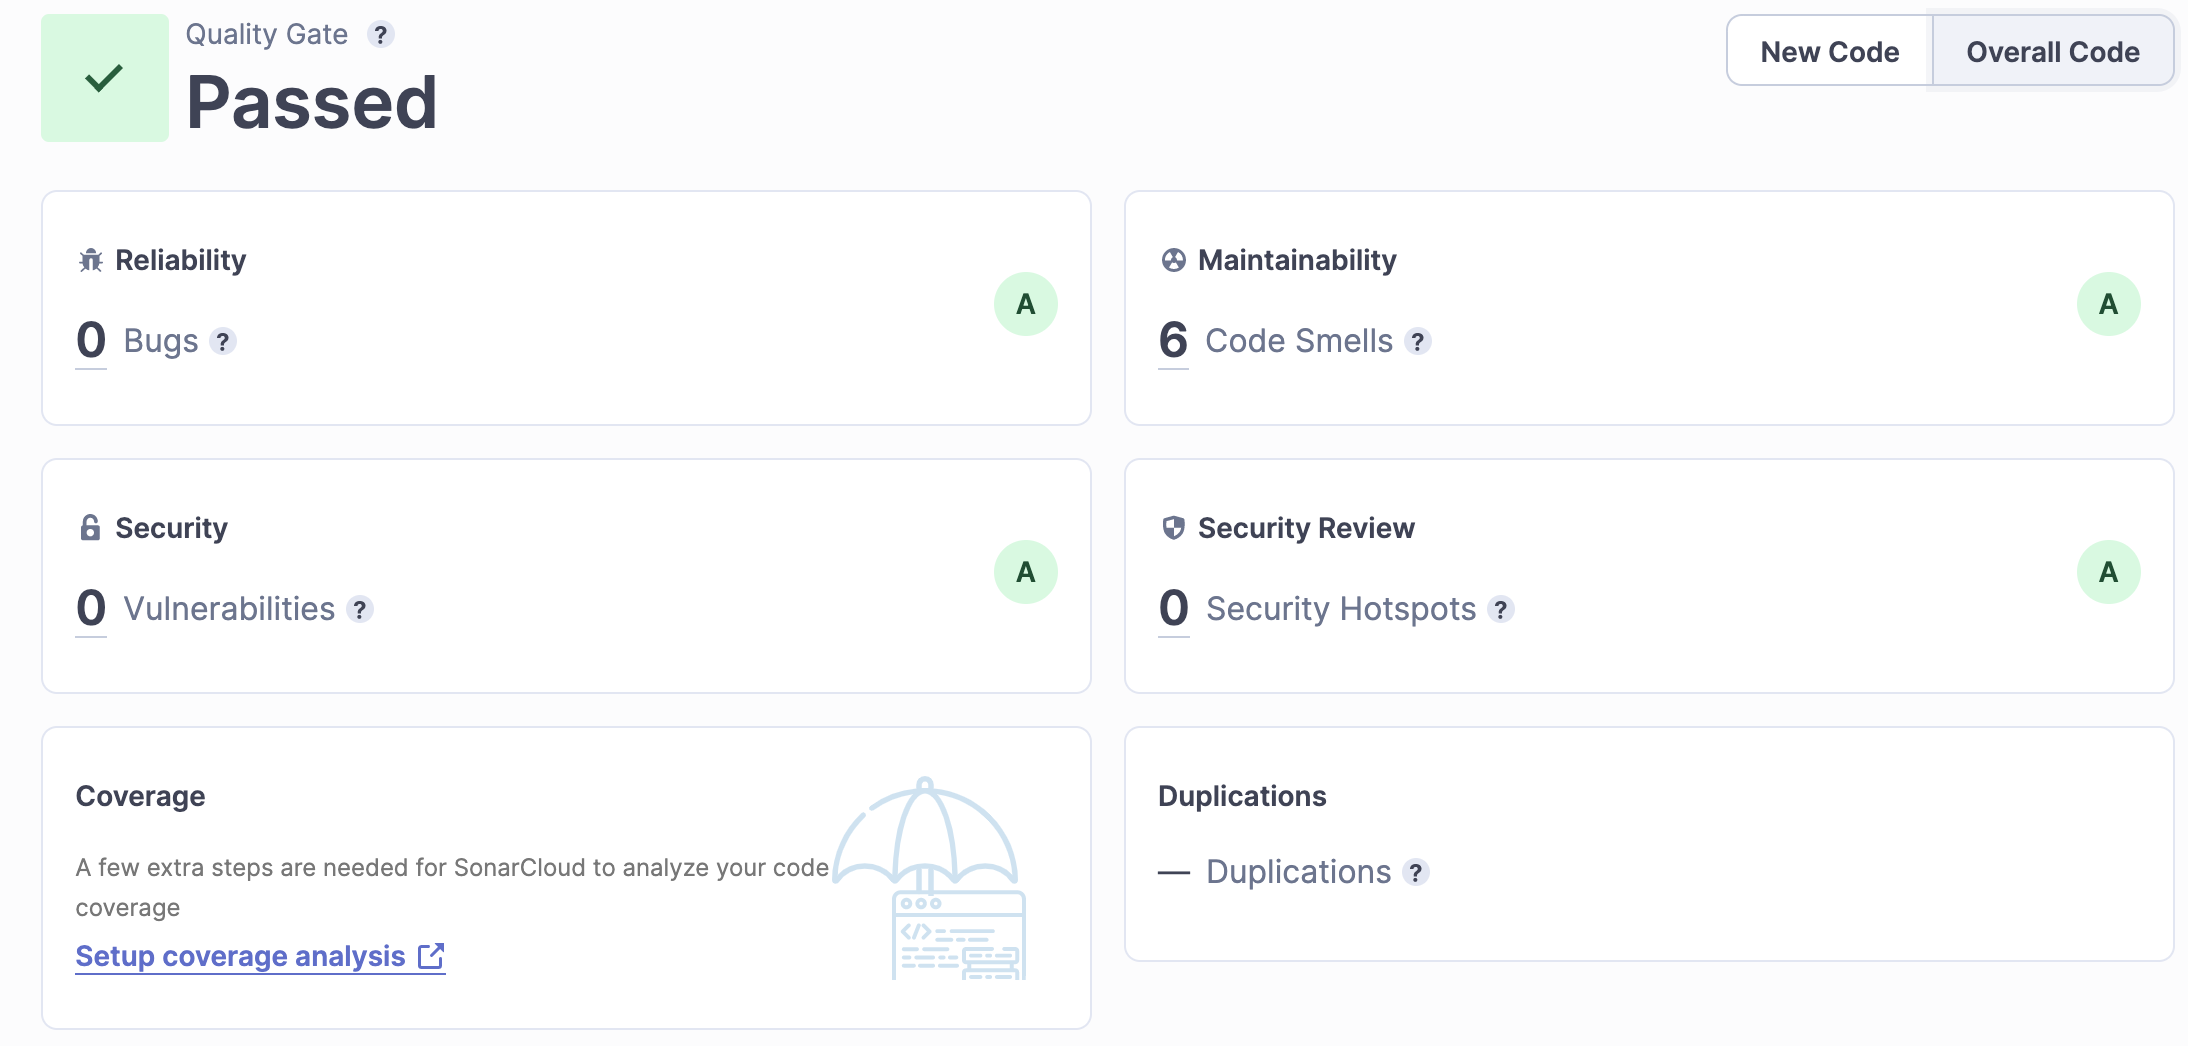
\includegraphics[width=\textwidth]{images/sonarcloud.png}
    \caption{Current state of the system}
    \label{fig:sonarcloud}
\end{figure}
\subsection{Licensing}
As there was no explicit license from the original Minitwit application we copied we see this program as our own minitwittware and therefore will have to license it ourselves. If we take a look at the denpendencies we use in the project and their licenses we see the following.
\begin{itemize}
    \item prometheus\\
    Apache 2.0 license
    \item grafana\\
    GNU AGPLv3 license
    \item SeriLog\\
    Apache 2.0 license
    \item ElasticSearch, Kibana and filebeat\\
    Elastic License and Server Side Public License (SSPL) (Elastic License v2, or ELv2) 
    \item nginx\\
    2-clause license ("Simplified BSD License" or "FreeBSD License"
    \item .NET (C\#)\\
    MIT license
    \item npgsql\\
    PostgreSQL License
    \item React\\
    MIT license
\end{itemize} 
Looking at the licences above the GNU AGPLv3 license seems like the strongest and since it is free it makes sense to go with the same\footnote{https://github.com/Group-O-Minitwit/minitwit-group-o/blob/main/LICENSE.md}. The GNU AGPLv3 is a strong copyleft license which we feel like makes sense for the project in case other people wants to help and make changes or use it as an inspiration for their own work then they have a starting platform.

\subsection{Technologies}
\label{technologies}
\subsubsection{Programming language and Framework}
For the backend we had to choose another language than python. This made our choice to quickly be between Go or C\# as we knew this were a course with a steep learning curve and we wanted the refactoring of the API for the application not take much time from other contents of the course. The reason for these two despite other recommendations was primarily the amount of documentation and resources available online when stuck on a problem\footnote{Stack Overflow 2022}.\\
The reason why we chose C\# over Go comes down to that most of us are more comfortable with the object oriented nature of C\# and it is an industry standard. By using this project as a portfolio project, it could make us more attractive for future job opportunities.\\

For the frontend we chose React.js. The choice for us here was either React or .NET's own frontend framework Blazor. Choosing Blazor would allow us to keep programming in C\# for the frontend.\\

The reason why we chose React and JavaScript over Blazor was because React already is used by Twitter, so for making a Twitter clone, it seems natural to use the same framework. React is also faster given it is browser native where as C\# uses web assembly. Again we also use the argument of attractiveness on the job market where very few applications are written in Blazor. Like C\#, React has gained a lot of following since its release, which makes it easy for us to find resources and documentation for the language.


\subsubsection{Virtualization techniques and deployment targets}
We have chosen to deploy our application on DigitalOcean as we as students get free credits and therefore didn't have to use any money ourselves. \\
As virtualization technique we have chosen to go with a droplet which has multiple containers which is all constructed through our \verb|docker-compose.yml| file\footnote{https://github.com/Group-O-Minitwit/minitwit-group-o/blob/main/remote\_files/docker-compose.yml}. \\

We have chosen not to go with Vagrant since it added a layer of unnecessary complexity and because our application is so small that there is not real reason for managing our VM. \\

Our deployment target is docker 20.10.21 with ubuntu 20.04 as this is the newest LTS of Ubuntu making it a safe deployment target.
Our implimentation with 
\subsubsection{ORM framework and DBMS}
For the Object Relation Mapping, we're using ASP.NET Core. This is a .NET library which allows us to easily create models which directly relate to the database and set up API endpoints. This framework is the obvious choice when you're creating an API closely related to a relational database. This was for some people a new technology, but since it is widely used\cite{brainspire}, it's always a good tool to know.

For the Database Management System (DBMS) we're using PostgreSQL\cite{postgresql}. This is partly because of how easy it is to set up, both with integrating with ASP.NET Core and with its standalone docker image. Another reason why we chose this management system is for it's data types. When working with C\#, it's very easy to directly transfer the standard types to the PostgreSQL types.

\section{Process' perspective}
\subsection{Developer interactions}
\label{dev-interactions}
For internal communication in the group we have created a Slack workspace to ask questions, arrange meetings and share documents. We have used Microsoft Teams to facilitate our meetings as teams is also used in the class and offers a more reliable platform for online meetings compared to Slack. 

We had biweekly scrum-like meetings Tuesday and Friday to give an update on what tasks you had done, what you had started on, and if you needed any help with an ongoing task.

We kept track of work in progress and future work by using GitHubs issues function. In the beginning of the project we also used the projects option as a sort of kanban board in order to track when the application was refactored and which steps where still needed. 

We have used pull requests in order to have some quality assurance and outside perspective of work when a task was done. A pull request to the main branch had to be approved by at least one other member before it could be merged.
\subsection{Team organization}
We are a team of 6 student developers each with different time schedules and therefore we have split us into smaller teams responsible for backend and frontend according to our schedules. We primarily made use of pair programming, to ensure some sparring, when developing new features. 
\subsection{Stages and tools included in the CI/CD chain}

In our CI/CD pipeline everytime there is a push to the main branch, the \verb|continous-deployment.yml| script\footnote{https://github.com/Group-O-Minitwit/minitwit-group-o/blob/main/.github/workflows/continous-deployment.yml} builds, delivers and deploys the application to DigitalOcean. This script contains multiple steps starting with running tests as we do not want to deploy faulty software. After the tests passes we build and push the backend and frontend to DockerHub. When this is done we configure the SSH and copy our files from the \verb|remote\_files| directory onto the server as it contains the \verb|docker-compose.yml|\footnote{https://github.com/Group-O-Minitwit/minitwit-group-o/blob/main/remote\_files/docker-compose.yml} and \verb|deploy.sh|\footnote{https://github.com/Group-O-Minitwit/minitwit-group-o/blob/main/remote\_files/deploy.sh} so that the server always has the latest files

\subsection{Repository organization}
We have decided to use github for our repo management. This is something we were encouraged to use and a free service that we also had experience with in advance. We have chosen a mono-repo approach as the project is not going to be so big that more repositories would be necessary. There could be arguments for a dual repo setup with a repo for the backend and another for the frontend but sticking to a single made more sense as the arguments for a poly-repo setup are not strong enough in the case of 2 repos over a single. This also helped keeping complexity to a minimal when we had to deploy to the server.
\subsection{Applied branching strategy}
\label{applied-strategy}
We used a version of the GitHub Flow\footnote{GitHub} strategy to manage our branches. This involves having our main branch, which is the code we release to the world, a Development branch where we would merge features in order to ensure nothing breaks in the grander scheme and finally we would create feature branches based on GitHub issues to implement features.
Using this branching strategy easily gives an overview of which issues are being worked on as the branches names are usually \verb|feature/issue-number/name-of-feature|

\subsection{Applied development process and tools supporting it}
We have decided to split up our work throughout the group. The group members would have different responsibilities for parts of the website such as frontend, backend etc. \\
The reason for this partitioning was because we all have different schedules, it would not be feasible for a team of 6 to be a part of everything. \\

To support our process we used the GitHub tools of creating issues as also written above in section \ref{applied-strategy}. Another tool we used at the start was the projects tool which is a kanban board as described in section \ref{dev-interactions}.

\subsubsection{How do we expect contributions to look like?} 
A contribution should only be allowed into the development branch if the code is written in a readable manner, is tested and solves an issue contained in the backlog. The contributions has to pass the github actions checks unless there could be made arguments for a failing check is redundant. This is to ensure that no feature of functionality, which could break the app, is deployed to the server.

\subsubsection{Who is responsible for integrating/reviewing contributions?}
Every member in the group is responsible for reviewing contributions but a contributor will request reviews from team members more knowledgeable about the code and issues.

\subsection{Monitoring}
Our MiniTwit application supports monitoring with Prometheus and Grafana as a dashboard. 
We configured the setting for Prometheous and Grafana in the the \verb|prometheus.yml|\footnote{https://github.com/Group-O-Minitwit/minitwit-group-o/blob/main/remote\_files/prometheus.yml} and the docker-compose file.
This allowed us to access Grafana, Prometheus, and their metrics, enabling us to build our dashboard.\\
Monitoring is an essential aspect of managing IT systems and applications, providing feedback on their performance and quality of service. In our MiniTwit application. Prometheus and Grafana allow us to perform white-box monitoring (Pfeiffer, 2023), focusing on what's inside the application. With Prometheus, we are able to check the performance of our application's responsiveness regarding HTTP requests to identify potential bottlenecks, performance issues, and trends.\\
In addition to monitoring responsiveness, we also tracked other metrics, including CPU time usage, garbage collector run time, maximum file descriptors, and remote read queries. Prometheus collected and stored these metrics from our application, which can be accessed using Prometheus's queries in Grafana. This integration with Grafana allowed us to visualize and analyze the metrics, providing valuable insights into the performance of our application.\\


\subsection{Logging}
To implement logging in our system, we decided to go with part of the EFLK stack. Namely, ElasticSearch, filebeat and Kibana and replacing Logstash with .NET’s own logging library called Serilog. With this setup we are logging all API activity so that we through Kibana can visualize all the data we get.

We decided to drop Logstash as it is has high resource consumption which is not desirable for our system where we can risk getting a lot of API calls due to a large amount of users.
\subsection{Security assessment}
The output from the Metasploit Framework's Web Application Scanning module (\verb|wmap_vulns|) after scanning a target IP address (157.230.79.99) for vulnerabilities in directories and files seems like there were no vulnerabilities found. The scanner tested various modules to check for SSL, web server, and file/directory vulnerabilities, but there were no positive results indicating that the target site was vulnerable to any of them.\\ 
Some of the tests did not receive a response from the target site, which could indicate that the site is blocking requests or the scanner is being detected and blocked. However, without further information or analysis, it's not possible to determine the exact reason why the site did not respond.\\
The output shows that the scanner found three directories (/Login/, /login/, and /register/) and two files (/register and /login) on the target. For each directory or file found, the scanner performed an HTTP GET request and received a response code.\\
The response codes are 405 (Method Not Allowed) for the directories, indicating that the HTTP method used (GET) is not supported for those directories. For the files, the response codes are 404 (Not Found), indicating that the files were found but could not be accessed.\\
Overall, the output suggests that the target has directories and files that may be of interest to an attacker, but the access to them is restricted.

\subsection{Applied strategy for scaling and load balancing.}
For scaling the application we decided to go with Docker swarm. Docker swarm is a framework that provides both scalability and reliability via replication and load balancing.
\subsubsection{Implementing scaling}
When using the application towards the end of the simulator we realized the performance was getting slower. This made sense since we hadn't really upgraded our remote server or performance within our application so far. This is of course not ideal.
We realized too late, that we actually weren't that far from utilizing horizontal scaling. We were already using docker-compose, and with some small changes to the compose file, it would be possible to use the \codeword{docker stack deploy ...} to deploy our system in a docker swarm environment.\\
Though because we realized this too late, we, unfortunately, did not get the pipeline to reflect these changes. Our plan was to increase the amount of replicas running the API, to hopefully allow more requests to process simultaneously.\\
\subsubsection{Implementing availability}
We, unfortunately, also did not get to implement availability scaling during the period of this project. To increase availability in our system we would need to ensure that our services are constantly running, which would be possible by replication. This is not only replicating the processes but also increasing the number of servers used. This could be done by having a \textit{hot and standby}\footnote{Lungu 2023} setup. The reason it would be necessary to have multiple servers would be to ensure that even if the power got shut off to the main server, it could be detected by a heartbeat process\footnote{This is a process running on separate setup, pining the system in intervals to check it's availability.}, and prompt the system to switch to the standby server.

\subsection{AI assistance}
%In case anybody has used AI assitant programming or report writing
AI assistance was not used in the context of refactoring the project. However AI assistance was used to a minimal level, in the form of a lookup tool. It was used to resolve mistakes made in the codebase, when actually developing, as a replacement to conventional searching on the web. No code has been directly copied from the AI tool into the codebase. It was solely used as a guideline to give an idea of how to resolve common errors prompted by the compiler. \\

Tools used includes Github Copilot\footnote{https://github.com/features/copilot}, and GPT-4\footnote{https://openai.com/product/gpt-4}.

\section{Lessons Learned Perspective}
Throughout the development of our project, we encountered various challenges and gained valuable insights.

\subsection{Evolution and refactoring}
\label{evo-refac}
When we started out the project, we chose to use ASP.NET and PostgreSQL, which is what we stuck with using. But we connected it in such a way that we wouldn't be able to migrate the database (i.e. change datatypes, alter tables, and such). We could fix this by recreating the database, but since the system was live, this was not an option for us. We ended up fixing it by carefully creating a backup, and with multiple steps, tricking the system into using the old database, but with the database being migratable. Due to this, the system was only down for about half an hour.\\

When developing our frontend, we ran into some issues, where our frontend would not send back the data to the API. This happened even though the information it got, which was formatted to json, seemed like it should work. We tried posting the same json to the API through postman wihtout any errors. We found out it was caused by the browser, which uses CORS (Cross-origin Resource Sharing\footnote{Mozilla}) a a security measure, to protect the user from potential attacks. We eventually used a proxy to bypass the CORS error. This is not an optimal solution, but we couldn't find any other solution, at the time. 

\subsection{Operation}
While we were always able to operate the simulator through the API, it took us quite a while to get a frontend running due the problems mentioned in section \ref{evo-refac} above.

\subsection{Maintenance}
The intricacies of continuous integration and deployment demand careful consideration from start to finish. This was made evident when we first embarked upon configuring our own CI/CD pipeline – the initial setup presented several difficulties. 
We soon realized that grasping how every component interconnects with others within the pipeline was key, alongside ensuring precise configuration throughout. We encountered some setbacks along the journey but found success by persevering through experimentation until resolving any corresponding troubles related to remote server deployment.


\section{Conclusion}
Ensuring the security and integrity of our application was a top priority throughout the development process. We recognized the importance of implementing monitoring systems and conducting thorough penetration testing to identify and mitigate potential vulnerabilities.

By using GitHubs tools to plan and organize our work we were able to closely monitor issue tracking and use an appropriate branching strategy to manage tasks holistically.

Furthermore, the intricacies of continuous integration and deployment required meticulous attention and precise configuration. We recognized the importance of understanding how each component is interconnected within the pipeline. By persevering and conducting thorough experimentation, we overcame challenges related to remote server deployment and established a reliable and efficient CI/CD pipeline.

In summary, our project has provided us with invaluable lessons in monitoring, security, scalability, and continuous integration and deployment. These lessons will undoubtedly shape our future projects and contribute to our professional growth as software developers. The project stands as a testament to our dedication and commitment to delivering high-quality solutions to real-world problems while prioritizing effective communication, meticulous planning, scalability, and security measures.

\nocite{*}
\newpage
\bibliographystyle{plain}
\bibliography{bib}

\end{document}
